%! TEX root = ../main.tex
% ==============================================================
% IMMUTABLE — generated automatically, do not edit this block
%
% — Provenance ───────────────────────────────────────────────────
%   script            : analysis_scratch/parallel_probe_agreement_bland_altman.py
%   computed_in       : analysis_scratch/parallel_probe_agreement_bland_altman.py (single-panel Bland-Altman variant of the 2x2 facet)
%   plot_type         : parallel_probe_agreement_bland_altman
%   data_class        : DELEG
%   generated_at      : 2026-05-07T17:18:01
%   findings_doc      : memory/methodology_*.md (parallel-probe section)
%
% — Thesis context ──────────────────────────────────────────────
%   chapter           : 04
%   caption_label     : fig:ch04_parallel_probe_agreement_bland_altman
%   caption_short     : 
%
% — Filters ────────────────────────────────────────────────────
%   panel             : full
%   wind              : 
%   amplitude [V]     : 
%   frequency [Hz]    : 1.3–1.6 Hz
%   probes            : 
%   run_category      : 
%   quality_flag      : ok
%   mooring           : 
%
% — Data provenance ────────────────────────────────────────────
%   n_runs            : 80
%   in_probes_used    : 9373/170+9373/340
%   out_probes_used   : 12400/250
%   probe_configs     : march2026_better_rearranging
%   non_final_config_n: 
%   datasets        :
%     (none registered — set plot_utils.ACTIVE_DATASETS)
%   run_paths       :
%     (omitted — aggregate over > threshold runs, see datasets)
%
% — Method / numerical parameters ─────────────────────────────
%   grouper           : 
%   collapse_panels   : 
%   fft_window_hz     : 
%   extra_params      : Single-panel Bland-Altman-style agreement plot pooling all 4 thesis frequencies (1.3, 1.4, 1.5, 1.6 Hz). x = (A_nær + A_fjern) / 2 [mm, FFT] where A_nær = Probe 9373/170 (wall-side) and A_fjern = Probe 9373/340 (far-side). y = (A_fjern - A_nær) / mean [%]. Same data scope as ch04_parallel_probe_agreement_by_freq (2 canon lowrange folders, panel=full, quality_flag=ok). Colour = WindCondition (no=blue, full=red). Marker = (amp tier × paddle freq) via wavescripts.plotter._freq_marker — outline shape is amp (○ A1, □ A2, △ A3), orientation/fill is freq (1.3 → 1.6 Hz). Reference bands: 0 % (perfect agreement, dashed), ±5 % (green fill), ±10 % (yellow fill).
%
% — Summary stats cited in caption ────────────────────────────
%   stat:n_runs_total : 80
%   stat:median_signed : -0.658 %
%   stat:max_abs_signed : 27.919 %
%   stat:std_signed   : 7.271 %
%   stat:n_runs_at_f13 : 30
%   stat:n_runs_at_f14 : 16
%   stat:n_runs_at_f15 : 16
%   stat:n_runs_at_f16 : 18
%
% — Subfigures available ───────────────────────────────────────
%     FIGURES/ch04_parallel_probe_agreement_bland_altman.pdf
% ── end immutable block ─────────────────────────────────────────
\begin{figure}[htbp]
  \centering
  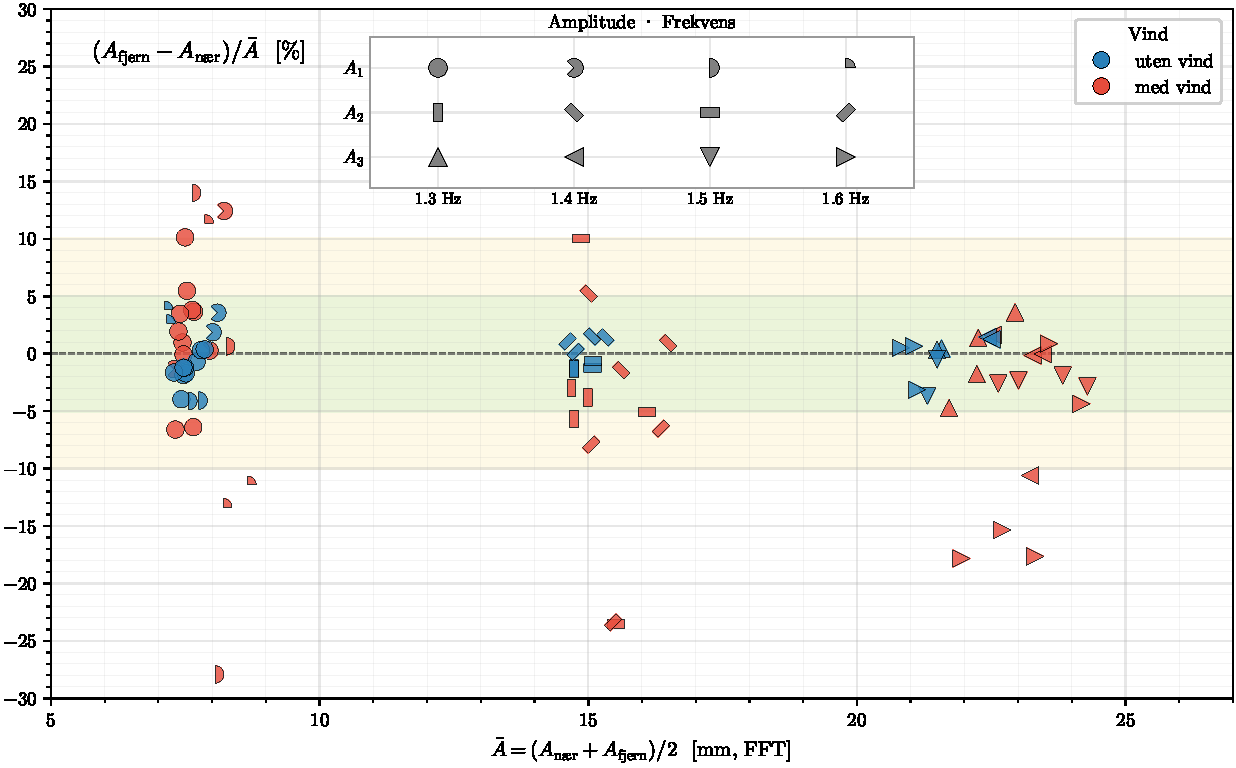
\includegraphics[width=\linewidth]{FIGURES/ch04_parallel_probe_agreement_bland_altman.pdf}
  \caption{
    Forskjell mellom parallelle prober. 
  }
  \label{fig:ch04_parallel_probe_agreement_bland_altman}
\end{figure}
